\documentclass[14pt,a4paper]{scrartcl}
\usepackage{cmap}
\usepackage[utf8]{inputenc}
\usepackage[T1,T2A]{fontenc}
\usepackage[english,russian]{babel}
\usepackage{relsize}
\usepackage{graphicx}
\usepackage{subfigure}
\usepackage{mathtools}
\usepackage{amssymb}
\usepackage{float}
\usepackage{sidecap}
\usepackage{wrapfig}
\usepackage{caption}
\usepackage[table,xcdraw]{xcolor}
\usepackage{listings}
\usepackage{minted}
\usepackage[hidelinks]{hyperref}

\begin{document}
	\begin{titlepage}
	\begin{center}
		\large
		МИНИСТЕРСТВО ОБРАЗОВАНИЯ И НАУКИ\\ РОССИЙСКОЙ ФЕДЕРАЦИИ
		
		\vspace{0.5cm}
		
		МГТУ им Н.Э.Баумана
		\vspace{0.25cm}
		
		Факультет ФН
		
		Кафедра вычислительной математики и математической физики
		\vfill
		
		
		Соколов Арсений Андреевич\\
		\vfill
		
		
		{\LARGE Домашнее задание №3 по математической статистике\\[2mm]
		}
		\bigskip
		
		3 курс, группа ФН11-53Б\\
		Вариант 9
	\end{center}
	\vfill
	
	\newlength{\ML}
	\settowidth{\ML}{«\underline{\hspace{0.7cm}}» \underline{\hspace{2cm}}}
	\hfill\begin{minipage}{0.4\textwidth}
		Преподаватель\\
		\underline{\hspace{3cm}} Т.\,В.~Облакова\\
		«\underline{\hspace{0.7cm}}» \underline{\hspace{1.71cm}} 2019 г.
	\end{minipage}%
	\bigskip
	
	
	\vfill
	
	\begin{center}
		Москва, 2019 г.
	\end{center}
\end{titlepage}

\section{Моделирование выборки методом обратных функций}
Пусть требуется получить значения случайной величины $X$, распределенной в интервале $(a;b)$ с плотностью вероятности $f(x)$.
Стандартный метод моделирования основан на том, что интегральная функция распределения $F(y) = \int\limits_a^x f(x) dx$ любой непрерывной случайной величины равномерно распределена в интервале $(0;1)$, т.е. для любой случайной величины $X$ с плотностью распределения $f(x)$ случайная величина равномерно распределена на интервале $(0;1)$.
Тогда случайную величину $X$ с произвольной плотностью распределения $f(x)$ можно рассчитать по следующему алгоритму, графическое решение которого представлено на Рис.~\ref{ris:graphical_solution}.
\begin{figure}[h]
	\center{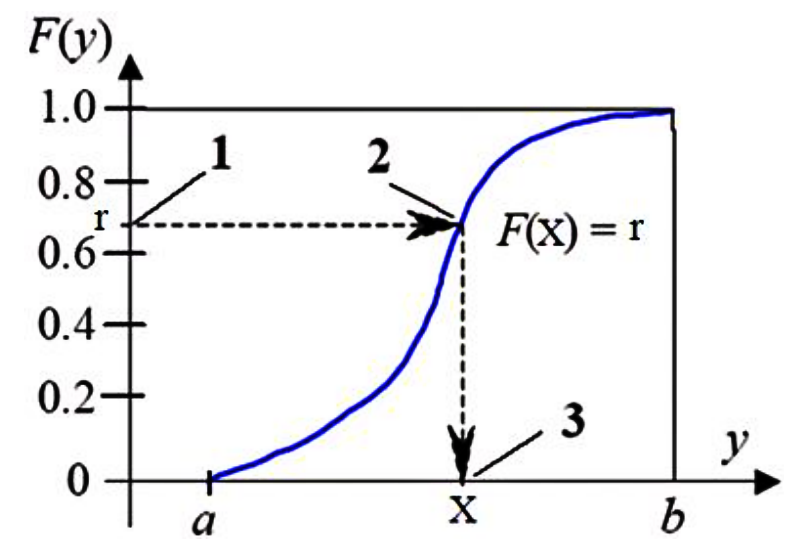
\includegraphics[width=0.7\linewidth]{../img/graphical_solution.png}}
	\caption{Графическое изображение метода обратных функций.}
	\label{ris:graphical_solution}
\end{figure}

\textbf{Алгоритм.}
\begin{enumerate}
	\item Необходимо сгенерировать случайную величину $r$ (значение случайной величины $R$), равномерно распределенную в интервале $(0;1)$.
	\item Приравнять сгенерированное случайное число известной функции распределения $F(X)$ и получить уравнение $F(y) = \int\limits_a^x f(x) dx = r$.
	\item Решая уравнение $X = F^{-1}(r)$, находим искомое значение $X$.

\end{enumerate}

Такой способ получения случайных величин называется \textit{методом обратных функций}.

\pagebreak
\textbf{Решение.}\\
По условию, имеется выборка, объёмом $n = 120$ элементов, подчиняющаяся логнормальному распределению с плотностью
\begin{equation*}
	p(x) = \frac{1}{\sqrt{2\pi} \sigma x} e^{-\frac{(\ln(x) - \mu)^2}{2\sigma^2}}
\end{equation*}
с параметрами $\mu = 2$ (mean value), $\sigma = \sqrt{0.2}$ (standard deviation).

Получим $n = 120$ случайных величин, равномерно распределенных на интервале $(0;1)$:
\begin{minted}{R}
> n <- 120
> 
> set.seed(1337)
> rand_vect <- runif(n, 0, 1)
> head(rand_vect, 5)
[1] 0.57632155 0.56474213 0.07399023 0.45386562 0.37327926
\end{minted}

Для генерации выборки методом обратных функций, воспользуемся функцией встроенной функцией, которая реализует  inverse cumulative distribution function (quantile function):
\begin{minted}{R}
> emp_sample <- qlnorm(rand_vect, meanlog = 2, sdlog = sqrt(0.2))
> emp_sample
[1]  3.990763 12.302612  8.497904  8.025929 12.197833  4.247885
[7]  9.124920 13.659752 12.235190  9.621277 10.005020  7.179212
[13] 14.518153  5.497928 18.573254  7.721113  5.524374  5.360958
[19]  4.086884  5.336768  9.923687  7.588191  6.692421  7.848874
[25]  4.805251  2.145636  8.035223  5.911119  7.429629 12.414112
[31] 10.160859  4.427855  5.274709  5.596016  7.516338  9.754663
[37] 12.515976  6.218515  6.899750  6.917922  6.873591 14.774747
[43] 14.197261  6.996216 18.149756  9.754281  7.135947  6.287228
[49] 13.540432  7.993637  4.667527  5.183359  4.638413  8.610529
[55]  5.006042  4.567935 10.821463  4.528023  5.592873  9.534546
[61] 12.726443 16.294013  3.578286  7.181449  7.165889  5.036149
[67]  7.183834  8.938177 11.954062  4.929206 12.242937  8.298037
[73]  9.036860  7.625875  7.558123  8.852263  6.989422  6.604355
[79] 11.110204  4.592310  8.116544  4.243953  6.220247  6.025850
[85] 13.646471  3.930147  7.933541  5.749459  6.742192 11.477393
[91]  5.047701  6.011809  5.144834  9.803677  9.379658 19.760923
[97]  7.619729  7.451011  5.314831  8.418257  5.990557 19.579448
[103]  5.464541  5.047026  5.307714  7.182732 12.621683 12.058664
[109]  8.748923  8.471951  8.355218  3.788953  4.931962  9.103708
[115]  8.855572  2.970164  6.639599  4.964537 11.946642  3.794012
\end{minted}

\section{Анализ полученной выборки}
Для анализа полученной выборки построим несколько графиков:
\begin{minted}{R}
>library(fitdistrplus)
> png(filename = "../img/graphics_1.png", 
+     width = 1920, height = 1080,
+     pointsize = 24, res = 96 * 1.25)
> plotdist(emp_sample, distr = "lnorm", list(2,sqrt(0.2)),
+          histo = T, demp = T)
> dev.off()

\end{minted}

\begin{figure}[h]
	\center{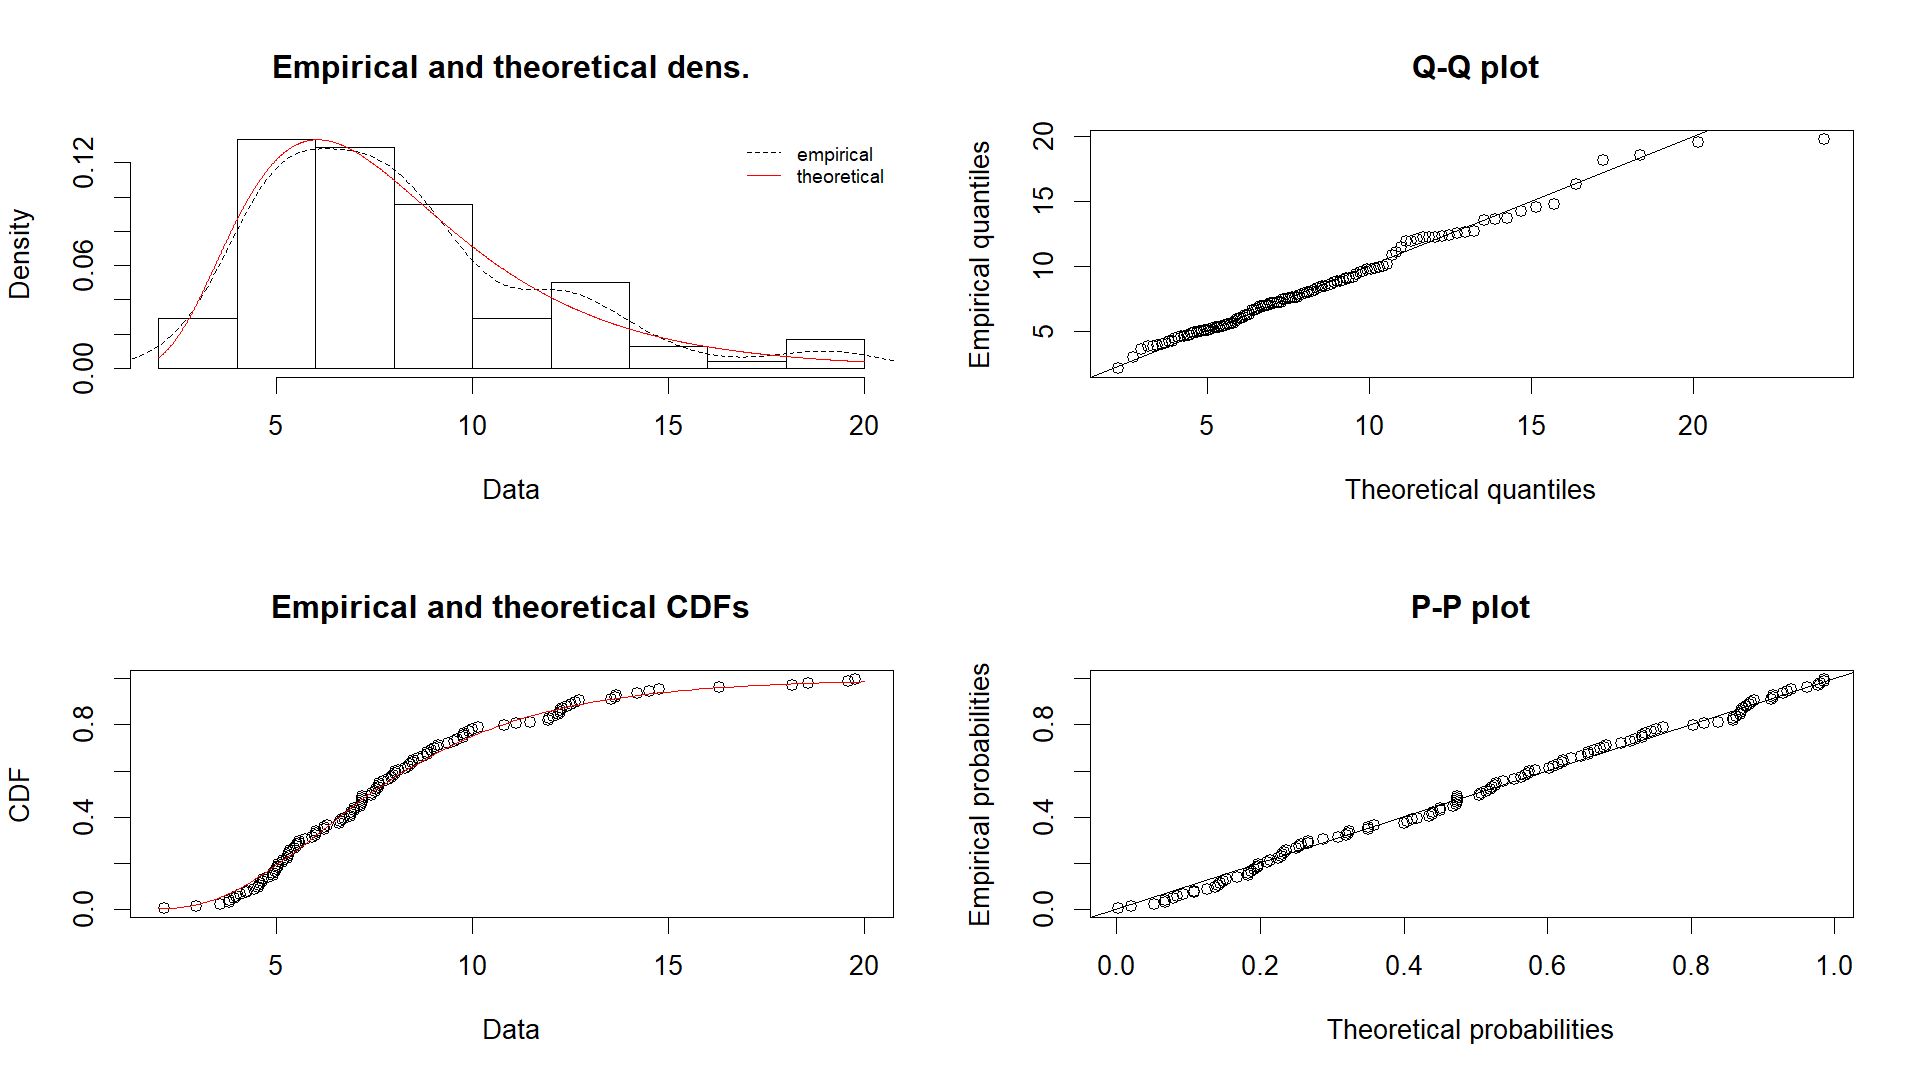
\includegraphics[width=1\linewidth]{../img/graphics_1.png}}
\end{figure}

А также вычислим среднее и стандартное отклонение для нашей выборки и сравним с теоретическими:
\begin{minted}{R}
> emp_mean <- mean(emp_sample)
> emp_mean
[1] 8.13665
> 
> theor_mean <- mean(theor_distr)
> theor_mean
[1] 8.195072
> 
> 
> emp_sd <- sd(emp_sample)
> emp_sd
[1] 3.563209
> 
> theor_sd <- sd(theor_distr)
> theor_sd
[1] 4.53649
\end{minted}


\section{Построение доверительного интервала функции распределения}
\subsection{Dvoretzky–Kiefer-Wolfowitz}
Существует несколько вариантов построения доверительной полосы (confidence band) для CDF. Один из них основан на неравенстве Дворецкого-Кифера-Вольфовица (ДКВ, Dvoretzky–Kiefer-Wolfowitz, 1956), которое определяет, насколько близко эмпирическая функция распределения связана с функцией распределения, из которой извлекаются эмпирические выборки:
\begin{equation*}
	\operatorname{Pr}\left(\sup \left|\hat{F}_{n}(x)-F(x)\right|>\epsilon\right) \leq 2 \exp \left(-2 n \epsilon^{2}\right),
\end{equation*}
где $\epsilon$ -- некоторая положительная постоянная.

Если принять уровень значимость $\alpha = 2 \exp (-2 n \epsilon^{2})$, то $\epsilon(n) = \sqrt{\frac{\ln(\frac{2}{\alpha})}{2n}}$. Используя  неравенство ДКВ и представленное выражение для $\epsilon$, можно оценить доверительные интервалы $(CI)$ для $F(x)$:
\begin{equation*}
	CI_{l,u} = \hat{F_n}(x) \pm \epsilon,
\end{equation*}
которые будут находиться на одинаковом удалении от каждой точки ECDF по оси ординат.

Более точно значение $\epsilon$ можно оценить с помощью аппроксимации статистики Колмогорова-Смирнова (КС) функцией approx.ksD() (Bickel \& Doksum, table IX,  p.483; Lienert G.A.(1975)) для доверительного уровня 0.95:

\begin{minted}{R}
> approx.ksD <- function(n) 
+ {
+   ## оценка критического значения статистики Колмогорова-
+   ## Смирнова D для доверительного уровня 0.95.
+   ## реализована по Bickel & Doksum, table IX,  p.483
+   ## и Lienert G.A.(1975) 
+   ifelse(n > 80, 1.358 /( sqrt(n) + .12 + .11/sqrt(n)),   ##B&D
+      splinefun(c(1:9, 10, 15, 10 * 2:8),# from Lienert
+                c(.975,   .84189, .70760, .62394, .56328,  # 1:5
+                  .51926, .48342, .45427, .43001, .40925,  # 6:10
+                  .33760, .29408, .24170, .21012,     # 15,20,30,40
+                  .18841, .17231, .15975, .14960)) (n))
+ }
\end{minted}

\subsection{Центральная предельная теорема}
Второй вариант основан на том, что согласно центральной предельной теореме (ЦПТ) асимптотическое поточечное распределение абсолютной разности $F(x)$ и $\hat{F_n}(x)$ имеет нормальное распределение со стандартной степенью приближения
\begin{equation*}
	\sqrt{n}\left(\hat{F}_{n}(x)-F(x)\right) \rightarrow \mathcal{N}(0, F(x)(1-F(x))).
\end{equation*}

Поскольку $E(\hat{F_n}(x)) = F(x)$, мы можем оценить доверительную полосу $F(x)$, имеющую переменное значение в каждой точке ECDF:
\begin{equation*}
	\hat{F}_{n}(x) \pm z_{\alpha} \frac{\hat{F}_{n}(x)\left(1-\hat{F}_{n}(x)\right)}{n}
\end{equation*}

Рассмотрим код для построения графика доверительных огибающих:
\begin{minted}{R}
> # Функция, формирующая доверительные интервалы ECDF
> get_df.ecdf <- function(x, level = 0.05) {
+   n <- length(x)
+   x.sort <- sort(x)
+   y <- (1:n)/n 
+   # CI по теореме Дворецкого-Кифера-Вольфовица (ДКВ)
+   epsilon = sqrt(log(2/level)/(2*n))
+   L = pmax(y - epsilon, 0)
+   U = pmin(y + epsilon, 1)
+   D <- approx.ksD(n)
+   U3 <- pmin(y + D, 1)
+   L3 <- pmax(y - D, 0)
+   # CI на основе центральной предельной теоремы (ЦПТ)
+   z <- qnorm(1-level/2)
+   U2 = pmin(y + z*sqrt(y*(1-y)/n ),1)
+   L2 = pmax(y - z*sqrt(y*(1-y)/n ),0)
+   data.frame(x=x.sort, y, L, U, L2, U2, L3, U3) 
+ }
> 
> # Формирование таблицы
> df.emp <- get_df.ecdf(emp_sample)
> 
> 
> # Создание графика
> library(ggplot2)
> 
> 
> png(filename = "../img/emp_cdfs_1.png", 
+     width = 1920, height = 1080,
+     pointsize = 24, res = 96 * 1.25)
> ggplot(df.emp, aes(x=x, y=y)) + 
+   # Эмпирические распределения
+   geom_line(aes(colour="Emperical CDF"),size=2) + 
+   # Заливаются области доверительных интервалов ДКВ
+   geom_ribbon(aes(ymin = L, ymax = U, 
+               fill = "Dvoretzky–Kiefer–Wolfowitz"), 
+               alpha = 0.5) + 
+   geom_line(aes(x = x, y = L3, 
+             colour = "KS approximation"), 
+             linetype = "3313", size = 1) +
+   geom_line(aes(x = x, y = U3, 
+             colour = "KS approximation"), 
+             linetype = "3313", size = 1) +
+   # Рисуются кривые доверительных интервалов ЦПТ
+   geom_line(aes(x = x, y = L2, 
+             colour = "Central limit theorem"), 
+             linetype = "dashed", size = 1) +
+   geom_line(aes(x = x, y = U2, 
+             colour = "Central limit theorem"), 
+             linetype = "dashed", size = 1) +
+   labs(x = 'Sample values',
+        y = 'CDF') +
+   theme_bw()
> dev.off()
\end{minted}

\begin{figure}[h]
	\center{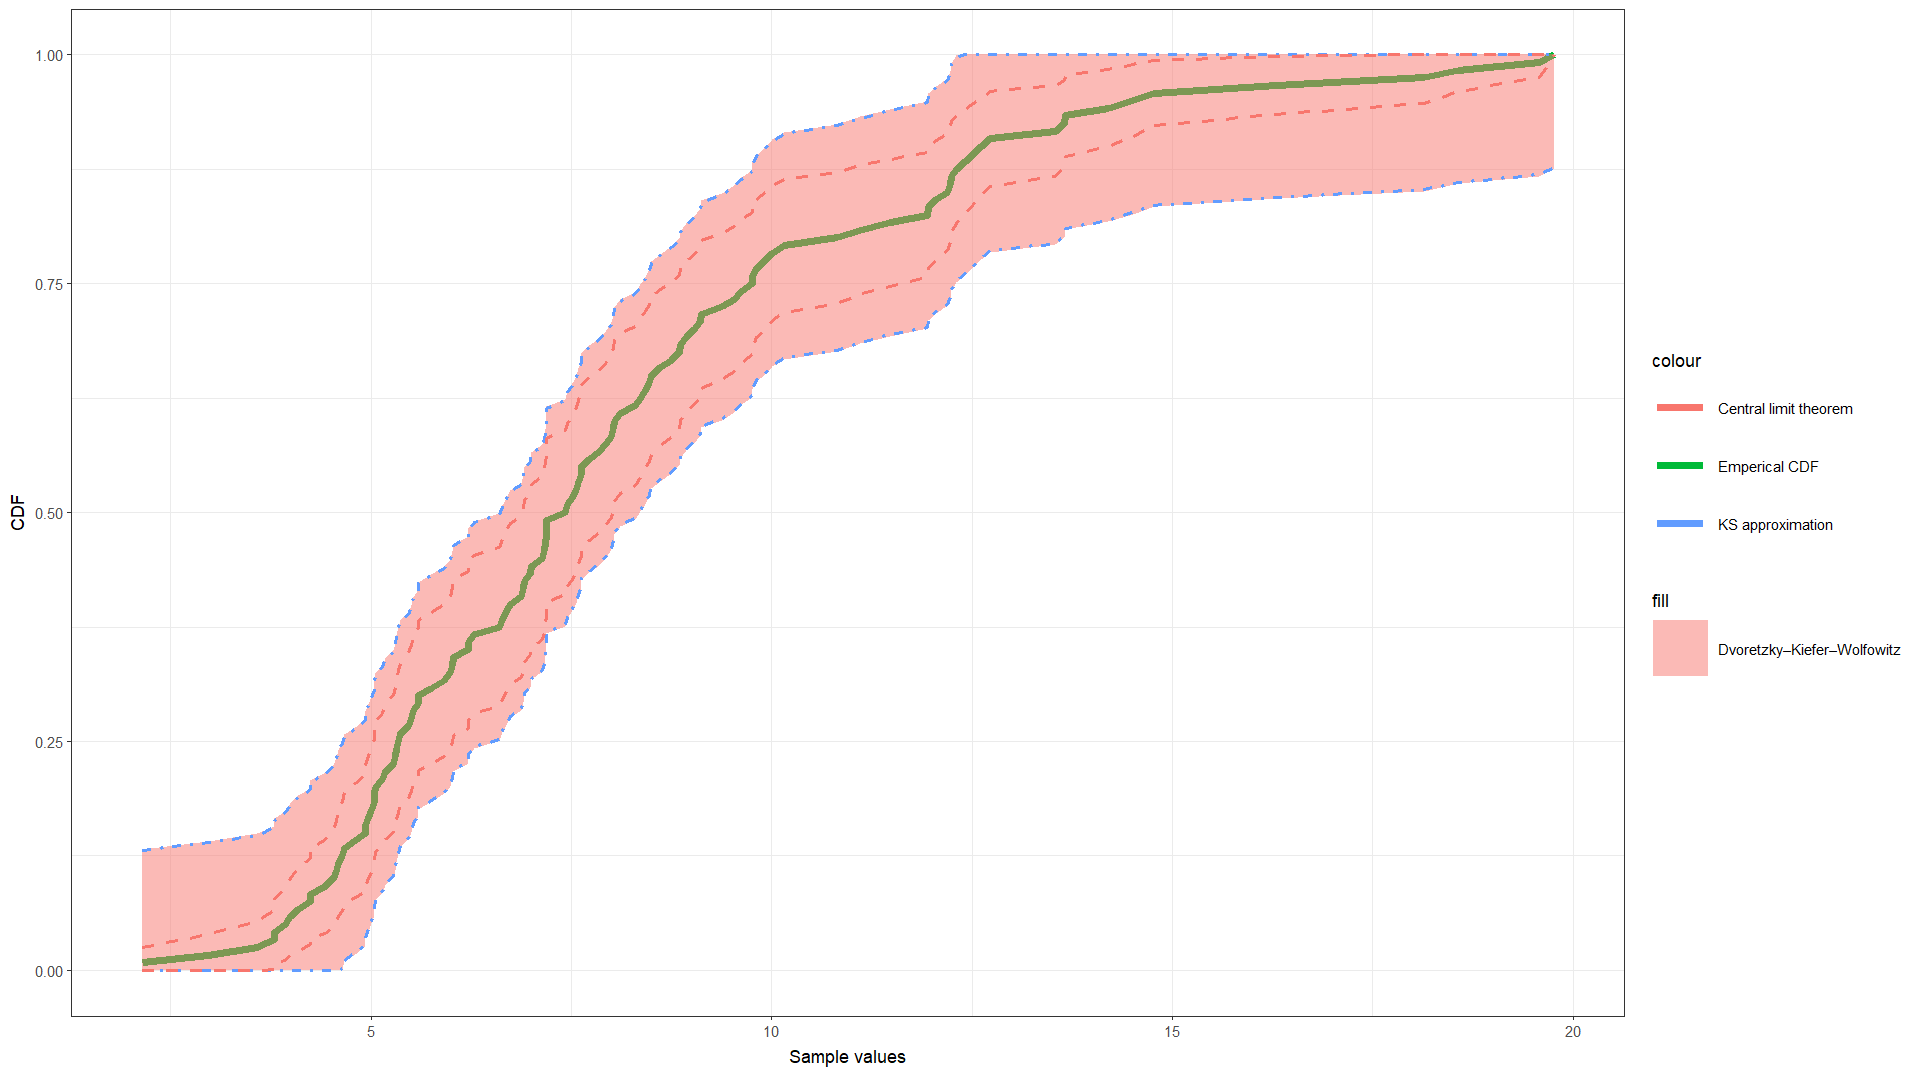
\includegraphics[width=1\linewidth]{../img/emp_cdfs_1.png}}
\end{figure}

\pagebreak
Здесь сплошной линией синего цвета показана эмпирическая CDF для нашей выборки с 95\% доверительной областью ДКВ, залитой прозрачно-красным цветом.  Штрих-пунктирной линией синего цвета отмечены границы, полученные с помощью аппроксимации КС, а штриховыми линиями красного цвета - полученные с применением ЦПТ.

\subsection{Бутстрэп}
Третьим способом оценки доверительных интервалов является непараметрическая бутстреп-процедура. Для этого на основе имеющейся эмпирической выборки генерируется множество псевдовыборок того же размера, состоящих из случайных комбинаций исходного набора элементов. При этом используется алгоритм "случайного выбора с возвращением" (random sampling with replacement), т.е. извлеченный выборочный элемент снова помещается в исходную совокупность, прежде чем извелекается следующее наблюдение. В результате некоторые наблюдения в каждой отдельной бутстреп-выборке могут повторяться два или более раз, тогда как другие - отсутствовать.

Для каждой бутстреп-выборки формируется кумулятивная функция распределения, а доверительная полоса в каждом ее вертикальном сечении включает "пучок" из 95\% таких кривых, максимально приближенных к медиане. Ограничимся 200 репликами:
\pagebreak

\begin{minted}{R}
> n = length(emp_sample)
> nrep = 200
> 
> # новые данные для построения плавной кривой
> newxs <- (seq(min(emp_sample), max(emp_sample), length.out = 100))
> 
> # добавление в итоговую таблицу координат ECDF
> pdat <- data.frame(newxs, py = ecdf(emp_sample)(newxs))
> 
> # создание бутстреп-выборок
> boots <- t(replicate(nrep, 
+                      emp_sample[sample.int(n, replace = TRUE)]))
> bootdat <- data.frame(apply(boots, 1, function(x) ecdf(x)(newxs))) 
> 
> # извлечение доверительных интервалов
> cis <- apply(bootdat, 1, quantile, c(0.025, 0.975))
> rownames(cis) <- c('lwr', 'upr')
> 
> # добавление доверительных интервалов
> pdat <- cbind(pdat, t(cis))
> 
> # таблица бустреп-кривых
> bootdat$newxs <- newxs
> require(reshape2)
> bootline <- melt(bootdat, id = 'newxs')
> 
> # Вывод итогового графика с использованием пакета  ggplot2
> png(filename = "../img/emp_cdfs_2.png", 
+     width = 1920, height = 1080,
+     pointsize = 24, res = 96 * 1.25)
> ggplot()+
+   labs(x = 'Sample values', y = 'CDF')  + 
+   geom_line(data = bootline, aes(x = newxs, y = value,
+             group = variable), col = 'steelblue', 
+             alpha = 0.5) +
+   geom_smooth(data = pdat,  aes(x = newxs, y = py), 
+               col = 'red', size=1.2, se= FALSE) +
+   geom_smooth(data = pdat, aes(x = newxs, y = lwr), 
+               linetype = 'dashed', size=1.2, se= FALSE) +
+   geom_smooth(data = pdat, aes(x = newxs, y = upr), 
+               linetype = 'dashed', size=1.2, se= FALSE) +
+   geom_smooth(data = df.emp, aes(x = x, y = L), 
+               linetype = '3313', col = 'green',size=1, se= FALSE) +
+   geom_smooth(data = df.emp, aes(x = x, y = U), 
+               linetype = '3313', col = 'green',size=1, se= FALSE) +
+   theme_bw()
> dev.off()
\end{minted}

\begin{figure}[h]
	\center{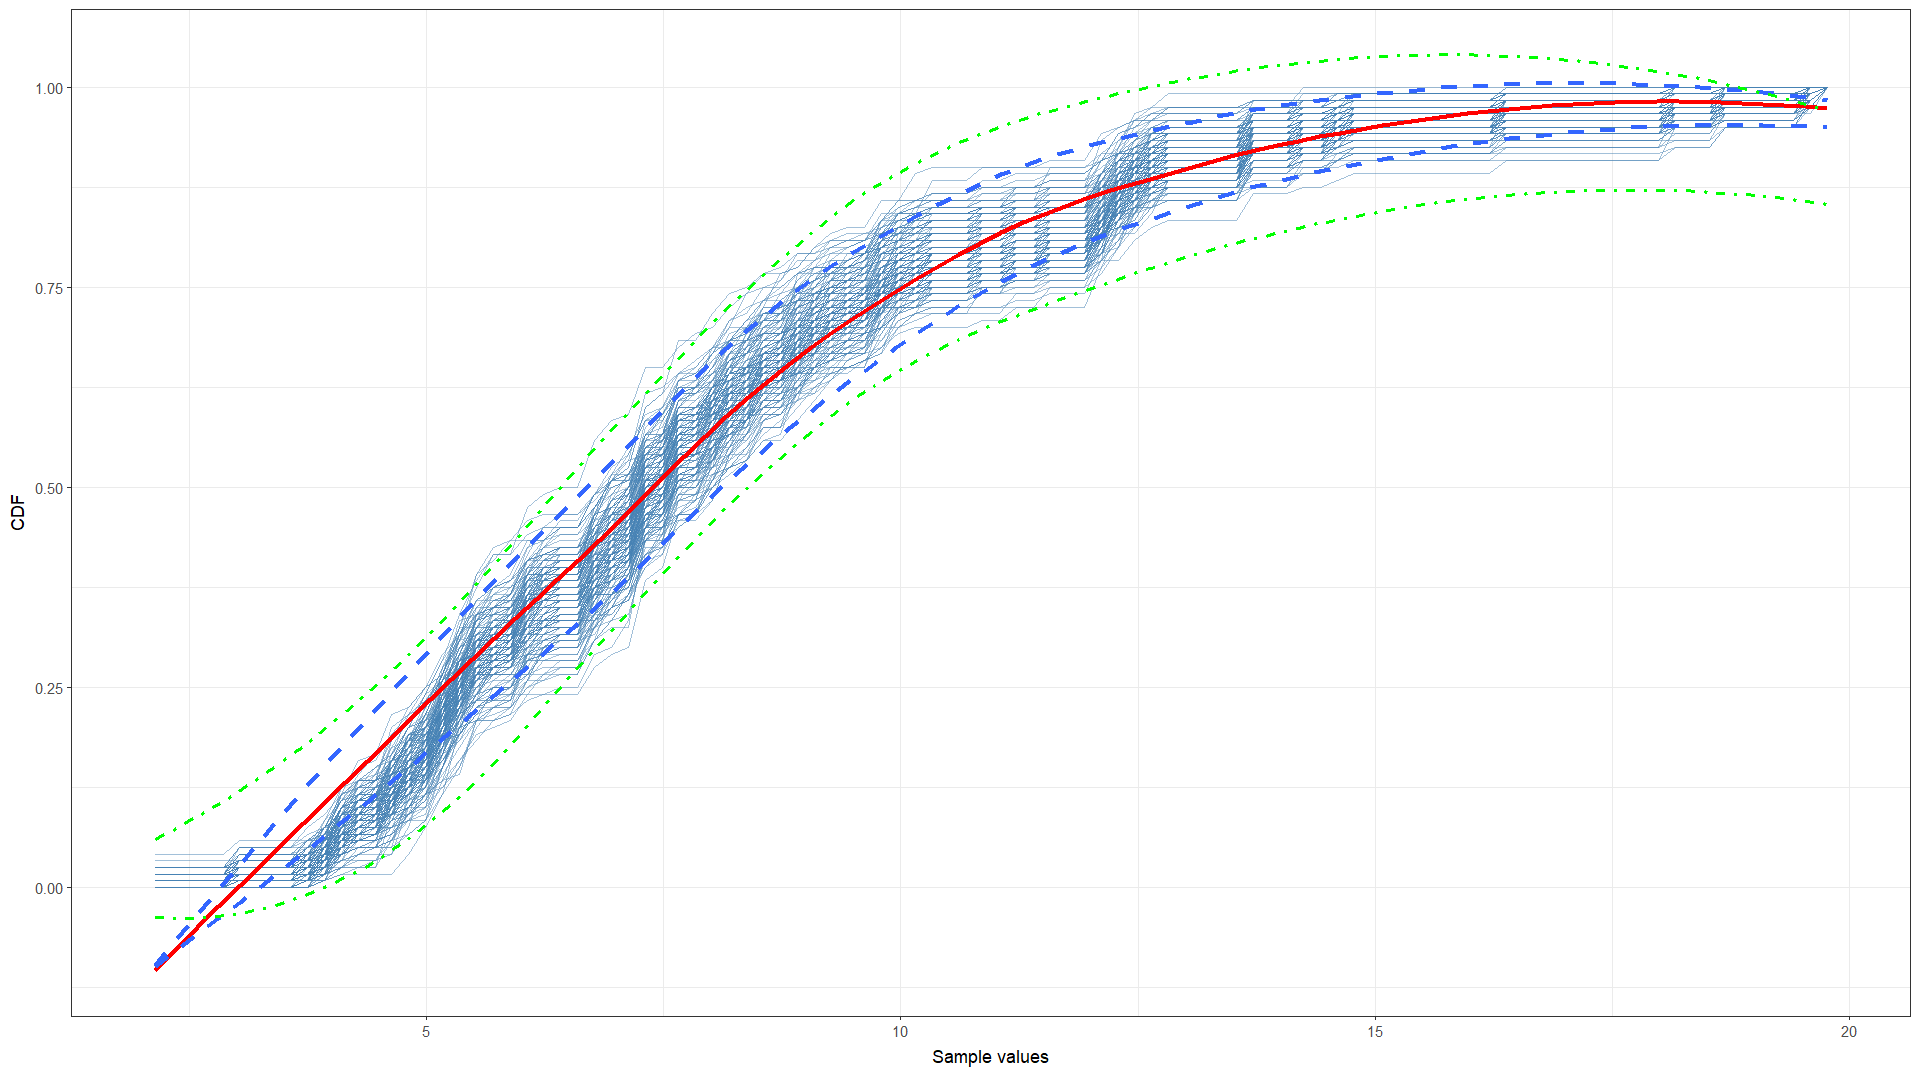
\includegraphics[width=1\linewidth]{../img/emp_cdfs_2.png}}
\end{figure}


Здесь ступенчатыми линиями показаны CDF на основе бутстреп-выборок. Остальные представленные кривые были сглажены локальной регрессией, в том числе: красным цветом показана эмпирическая CDF, синие штриховые линии обозначают доверительные огибающие, полученные бутстреп-методом, а зеленые штрих-пунктирные - доверительные огибающие, полученные из неравенства Дворецкого-Кифера-Вольфовица (приведены для сравнения).


Видно, что доверительные области, построенные на основе ЦПТ и бутстреп-метода существенно уже, чем ДКВ-области, особенно на обоих концах кумулятивной кривой. Как следует из дискуссии\footnote{\url{https://stats.stackexchange.com/questions/181724/confidence-intervals-for-ecdf}}, это - два разных типа доверительных полос. "Точечная доверительная полоса" (pointwise confidence band) предполагает, что, если выборки данных извлекаются из некоторого генерального распределения, то в среднем 5\% точек окажется вне доверительной области. Для "одновременной полосы" (simultaneous band) формулируется принципиально иное условие: существует 5\%-ная вероятность того, что точка с наибольшим отклонением окажется вне доверительной области (Francisco-Fernandez \& Quintela-del-Rio 2016).









\end{document}